\documentclass[main.tex]{subfiles}

\begin{document}

\subsection{Network statistico tra specie vegetali e specie entomologiche nei siti dell'Emilia-Romagna}

L’analisi del network tra specie vegetali ed entomologiche pronubi nei siti ERAI/ERESP dell’Emilia-Romagna ha definito, tramite le funzioni contenute nel pacchetto indicato precedentemente (Cap. \ref{Cap. 2.11}), i seguenti risultati.
I seguenti grafici esprimono le interazioni del network pesato tra apoidei e piante, correlando le bande superiori (piante) con le bande inferiori (apoidei). Lo spessore delle bande è proporzionale al numero di interazioni rilevate tra le parti mentre le linee esprimono l’intensità dei collegamenti tra esse. In particolare, il grafico relativo al sito denominato ERAI (Fig. \ref{fig:Interconnessioni ERAI}) definisce le interazioni tra le parti che avvengono nell’agroecosistema intensivo mentre il sito contrassegnato come ERESP (Fig. \ref{fig:Interconnessioni ERESP}) definisce le interconnessioni proprie dell’agroecosistema seminaturale.

\begin{figure}[H]
\centering
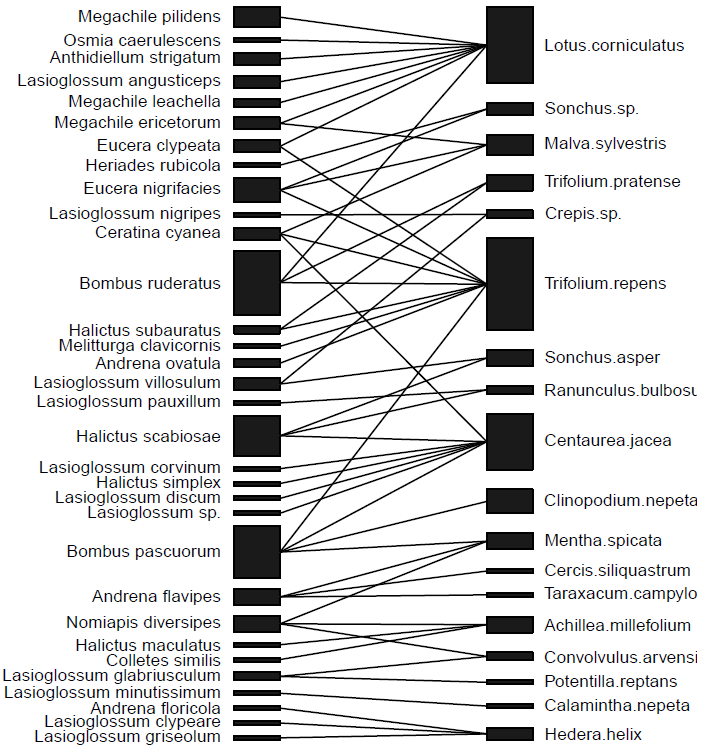
\includegraphics[width=0.85\textwidth]{./Immagini/Plotweb_Network_Api_Piante_AI.png}
\caption{Interconnessioni tra piante e impollinatori nel sito ERAI.}
\label{fig:Interconnessioni ERAI}
\end{figure}

\begin{figure}[H]
\centering
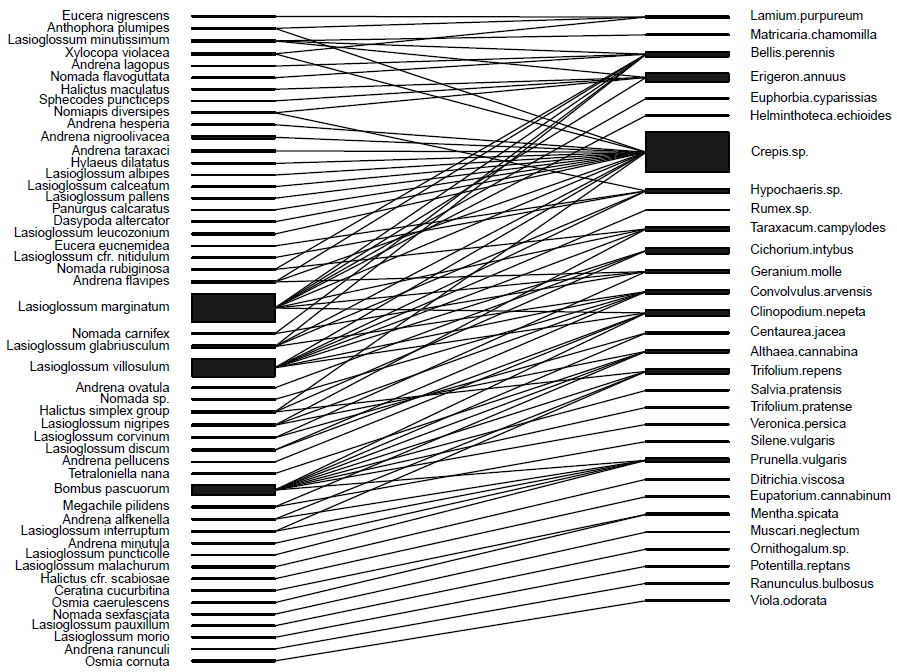
\includegraphics[width=1\textwidth]{./Immagini/Plotweb_Network_Api_Piante_ESP.png}
\caption{Interconnessioni tra piante e impollinatori nel sito ERESP.}
\label{fig:Interconnessioni ERESP}
\end{figure}

Un’ulteriore tipologia di visualizzazione esprime il network sotto forma di matrice grigliata, il cui gradiente di colorazione della cella rappresenta l’intensità dell’interazione tra impollinatore e pianta. Le celle con colori scuri indicano una forte interazione tra le parti mentre i colori chiari denotano una scarsa o assente interazione. Anche in questo caso i grafici definisco la rete piante-impollinatori per il sito intensivo ERAI (Fig. \ref{fig:grigliato ERAI}) e seminaturale ERESP (Fig. \ref{fig:grigliato ERESP}).

\begin{figure}[H]
\centering
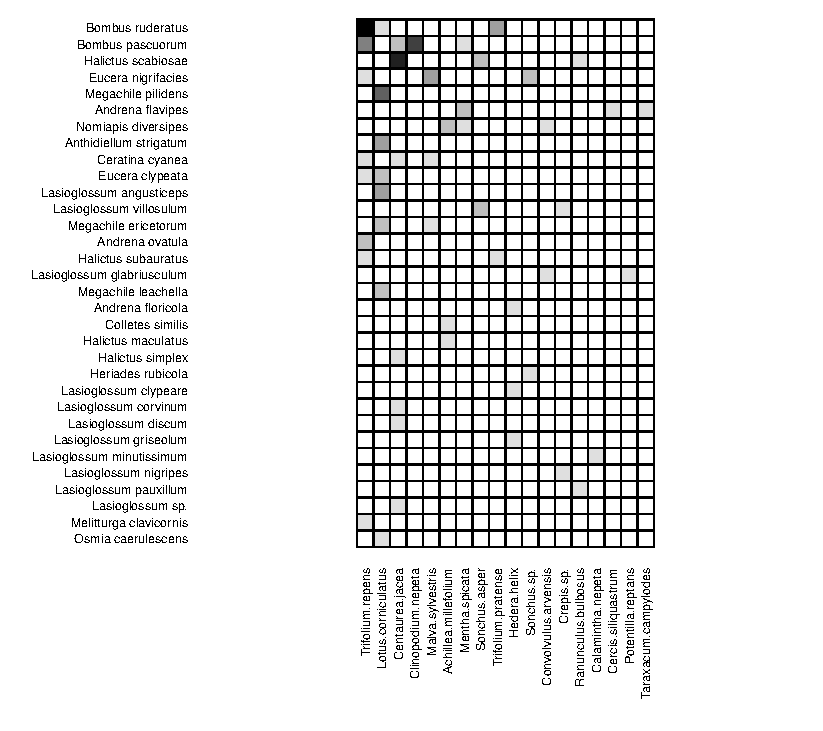
\includegraphics[width=1.2\textwidth]{./Immagini/visweb_Network_Api_Piante_AI.pdf}
\caption{grafico grigliato del network piante e impollinatori del sito ERAI.}
\label{fig:grigliato ERAI}
\end{figure}

\begin{figure}[H]
\centering
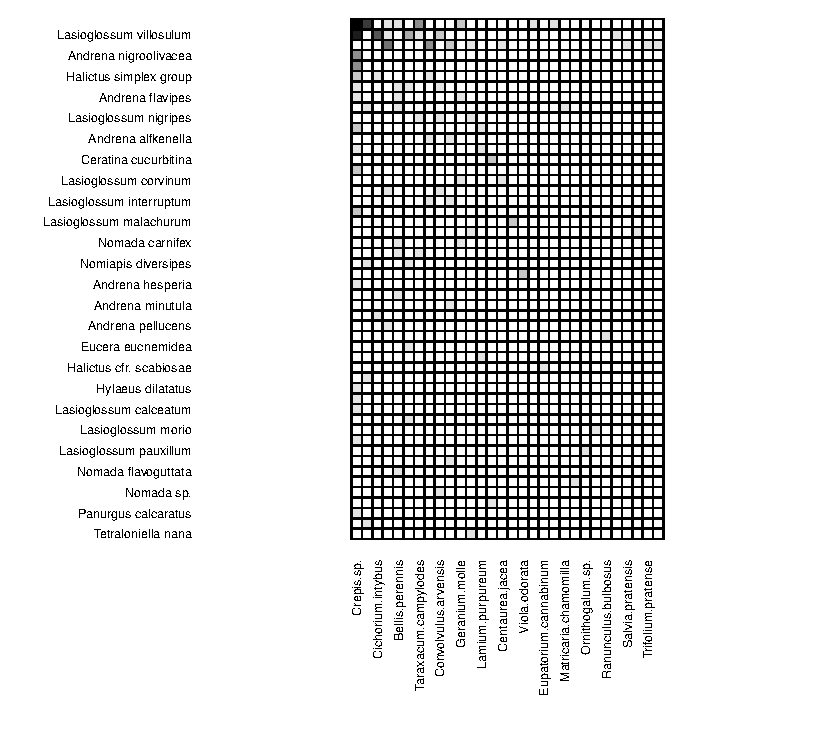
\includegraphics[width=1.2\textwidth]{./Immagini/visweb_Network_Api_Piante_ESP.pdf}
\caption{grafico grigliato del network piante e impollinatori del sito ERESP.}
\label{fig:grigliato ERESP}
\end{figure}

I seguenti indici (Tab. \ref{tab:7}) sono utili per definire le comunità di studio, composte da piante entomofile e pronubi nei rispettivi agroecosistemi, nella loro interezza:

\begin{table}[h!]
    \centering
\begin{tabular}{|1|1|1|}
\hline
~ & Agroecosistema intensivo (AI) & Agroecosistema seminaturale (ES)\\
\hline
modularity Q & 0.68799102 & 0.52705368 \\
\hline
Fisher alpha & 44.28707632 & 81.81804837 \\
\hline
Shannon diversity & 3.63724646 & 3.99898038 \\
\hline
\end{tabular}
    \caption{indici relativi all’intero network piante-impollinatori.}
    \label{tab:7}
\end{table}

A differenza degli indici precedentemente citati, le presenti metriche (Tab. \ref{tab:8}) invece definiscono la comunità di interesse a livello di gruppo:

\begin{table}[h!]
    \centering
\begin{tabular}{|1|1|1|}
\hline
~ & Agroecosistema intensivo (AI) & Agroecosistema seminaturale (ES)\\
\hline
Number of species HL & 18.00000000 & 30.00000000 \\
\hline
Number of species LL & 32.00000000 & 50.00000000 \\
\hline
Mean number of links HL & 5.31313131 & 8.74850299 \\
\hline
Mean number of links LL & 2.39393939 & 4.79640719 \\
\hline
\end{tabular}
    \caption{indici separati relativi sia al network composto da piante che da impollinatori.}
    \label{tab:8}
\end{table}

\end{document}





